\begin{frame}{Classical fANOVA Decomposition} % What is it?
  \begin{block}{General Form}
    \[
      y(\boldsymbol{X}) = \sum_{u \subseteq \{1,\dots,N\}} y_{u}(\boldsymbol{X}_u) = y_{\emptyset} + y_{\{1\}}(\boldsymbol{X}_1) + \dots + y_{\{1, 2\}}(\boldsymbol{X_1, X_2}) + \dots
    \]
  \end{block}
  \begin{itemize}
    \item $y$ : Model output
    \item $y_u$ : Component functions for subset $u$
    \item Assumption: $X_1, \dots, X_N$ are independent
  \end{itemize}
\end{frame}

\begin{frame}{Conditions for Classical fANOVA} % What conditions do we need?
  \begin{block}{Strong Annihilating Conditions}
    \[
      \int_{\mathbb{R}} y_u(\boldsymbol{x}_u) f_{\{i\}}(x_i) \, d\nu(x_i) = 0 \quad \text{for} \ i \in u \neq \emptyset.
    \]
  \end{block}
  \begin{itemize}
    \item Ensures unique component functions
    \item Applies under independent (product-type) input distributions
  \end{itemize}
\end{frame}

\begin{frame}{Key Properties}
  \[
    \mathbb{E}[y_u(\boldsymbol{X}_u)] = 0
  \]
  \[
    \mathbb{E}[y_u(\boldsymbol{X}_u) y_v(\boldsymbol{X}_v)] = 0 \quad (u \neq v)
  \]
  \begin{itemize}
    \item Zero mean components
    \item Mutual orthogonality
  \end{itemize}
\end{frame}

\begin{frame}{Component Construction} % How do we construct it?
    \[
    y_{\emptyset} = \int_{\mathbb{R}^N} y(\boldsymbol{x}) \prod_{i=1}^{N} f_{\{i\}}(x_i) \, d\nu (x_i) = \mathbb{E}[y(\boldsymbol{X})].
    \]
    \[
      y_u(x_u) =
        \int y(x) f_{-u}(x_{-u}) dx_{-u}
        - \sum_{v \subset u} y_v(x_v)
    \]
  \begin{itemize}
    \item $f_{-u}$ : marginal density of variables not in $u$
    \item Components solved sequentially by increasing order
  \end{itemize}
\end{frame}

\begin{frame}{Example: 2D Function} % How does it look?
  \begin{columns}
    \column{0.5\textwidth}
      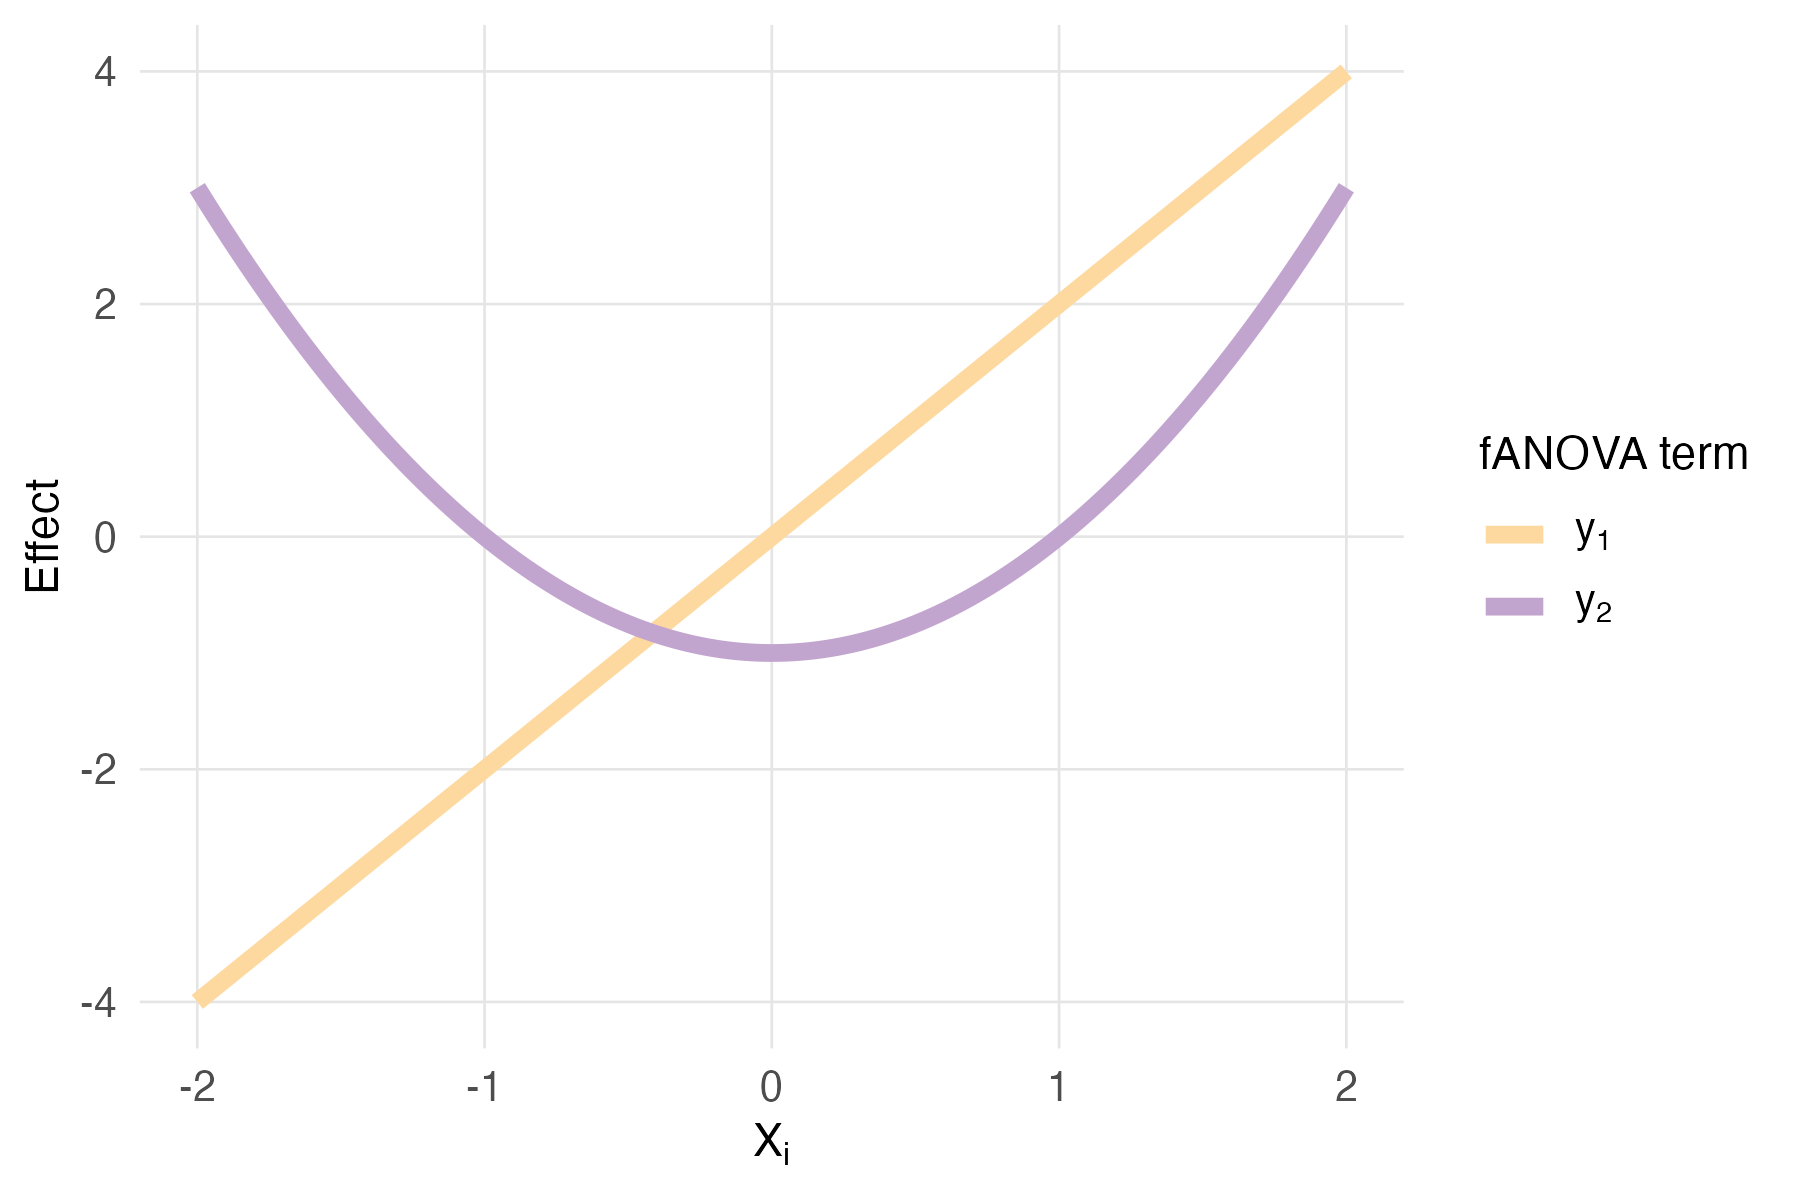
\includegraphics[width=\linewidth]{../images/experiment_section/classical_ex_1_a1p20_a2p00_a11p00_a22p10_a12p10_rhop00_main.png}
    \column{0.5\textwidth}
      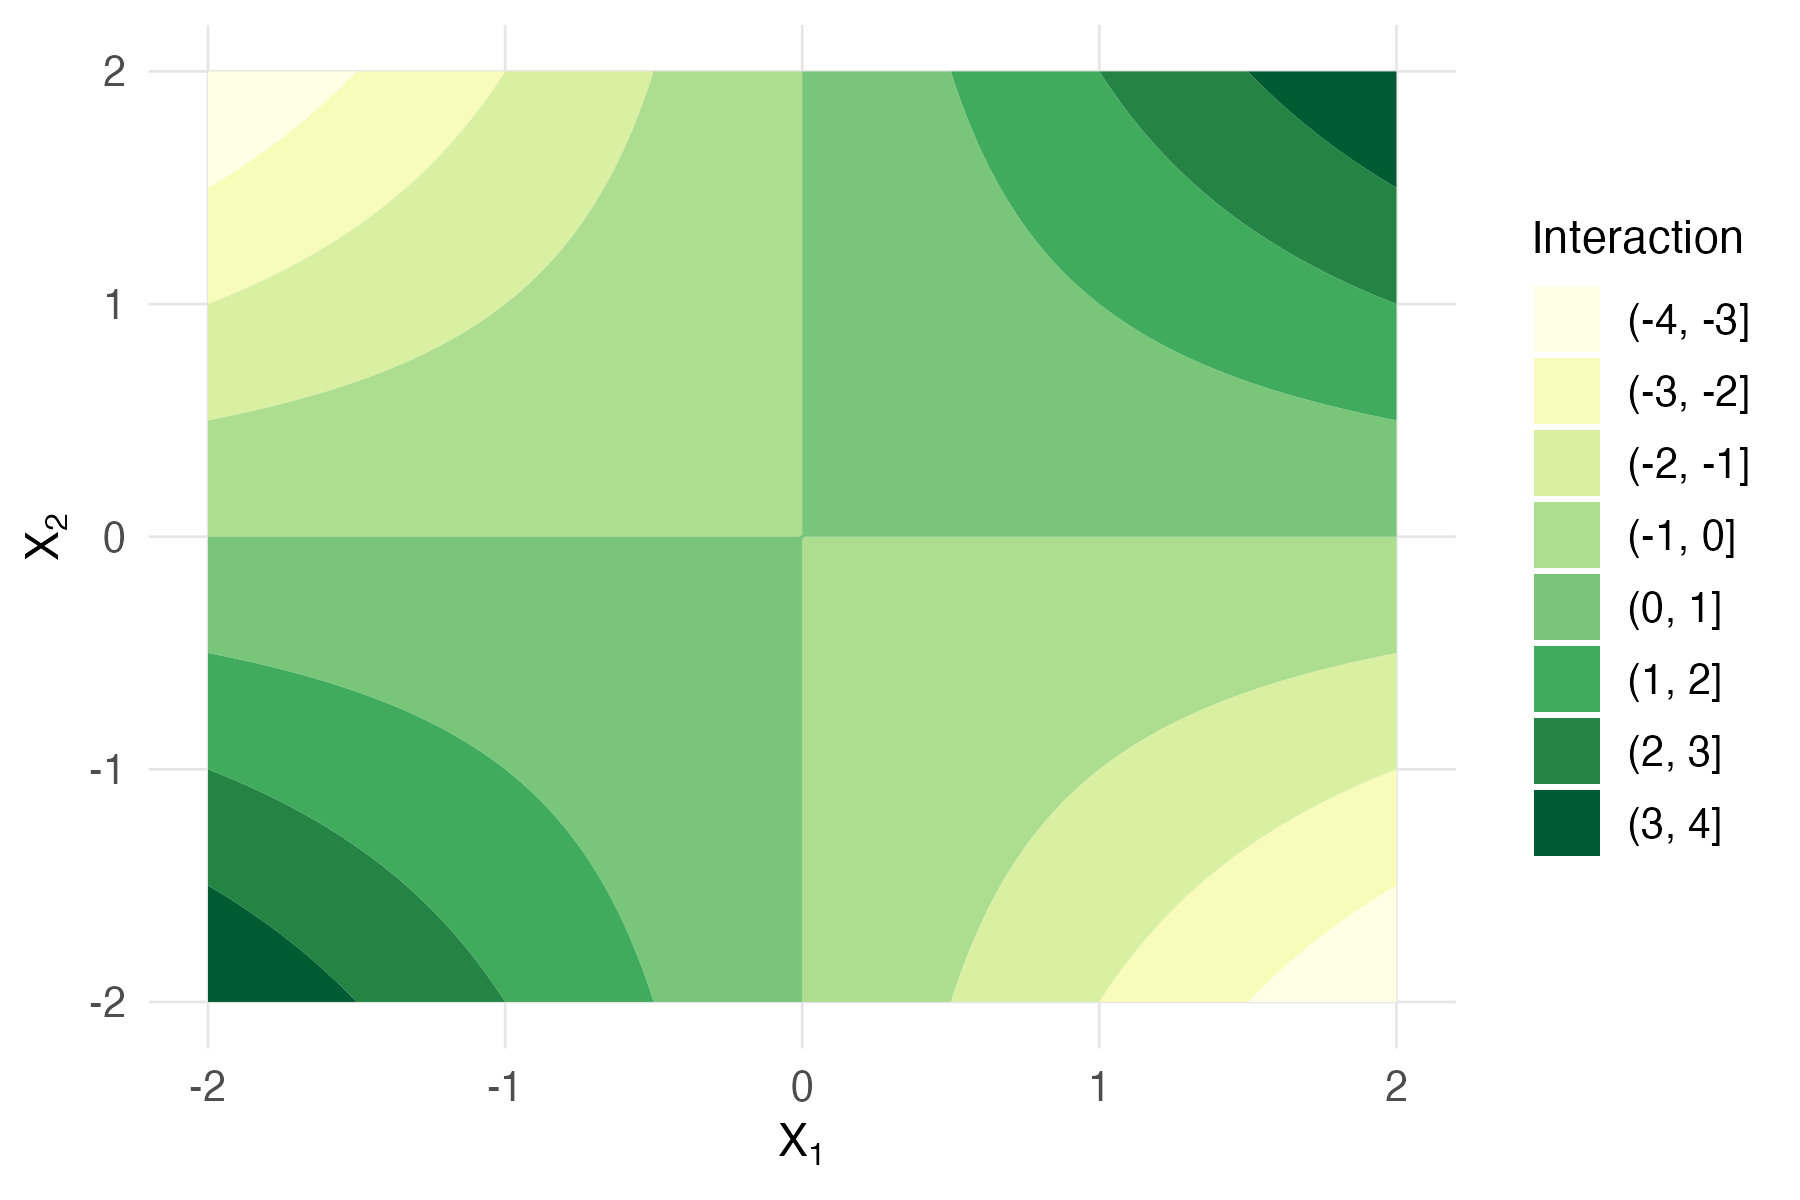
\includegraphics[width=\linewidth]{../images/experiment_section/classical_ex_1_a1p20_a2p00_a11p00_a22p10_a12p10_rhop00_interaction.png}
  \end{columns}
\end{frame}

% Equality to Hoeffding Decomposition


% fANOVA through lens of Orthogonal Projections
